\subsection{Lancer le logiciel d'acquisition}
\begin{enumerate}
    \item Allumer la caméra: mettre l'interrupteur \textit{Power} de \textit{Off} à \textit{On} (voir figure~\ref{fig:cam_power}).
        \begin{figure}[H]
        \centering
        \includegraphics[width=10cm]{cam_power.png}
        \caption{Interrupteur de la caméra}
        \label{fig:cam_power}
        \end{figure}
    \item Ouvrir l'ordinateur Mac.
    \item Entrer dans le compte \textit{dcclab} avec le mot de passe \textit{microscope}.
    \item Ouvrir le logiciel \textit{Umoco} (voir figure~\ref{fig:umoco}). Il y a un raccourci dans la barre de tâches et un autre sur le bureau.
        \begin{figure}[H]
        \centering
        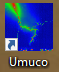
\includegraphics[width=2cm]{umoco.PNG}
        \caption{Raccourci du logiciel \textit{Umoco}}
        \label{fig:umoco}
        \end{figure}
    \item Sur l'interface d'accueil (voir figure~\ref{fig:accueil}), cliquer sur \textit{Camera}. Il est possible que le bouton \textit{Camera} ne soit pas encore disponible: il suffit d'attendre quelques minutes, le temps que le logiciel \textit{Umoco} détecte la caméra.
    \item Mettre \textit{Sensor mode} sur \textit{Area}.
\end{enumerate}